\chapter{Removing Waste}
\label{SoftwareEngineeringWasteChapter}
\section{Summary}

\textit{Context:} Software development is a complex socio-technical activity that involves coordinating different disciplines and skill sets and thus provides ample opportunity for waste to emerge. Waste is any activity that produces no value for the user.
\textit{Objective:} The purpose is to understand observed wastes in software development.
\textit{Method:} Following Constructivist Grounded Theory, we conducted a two-year participant-observation of several software development projects at Pivotal, interviewed \numberOfInterviews{} software engineers, interaction designers, and product managers, and analyzed one year of retrospection topics. We iterated between analysis and theoretical sampling until achieving theoretical saturation.
\textit{Results:}  This chapter introduces the first evidence-based waste taxonomy, identifying eight wastes along with causes and tensions within wastes. It also compares this study's taxonomy with the waste taxonomy found in Lean Software Development.
\textit{Limitations:} While the results are highly relevant to Pivotal, the outcomes might not apply to organizations with different software development cultures.
\textit{Conclusion:} The waste taxonomy serves as a starting point for waste identification and elimination. Comparing this taxonomy to Lean Software Development's list of wastes revealed our taxonomy's parsimony and expressiveness while illustrating wastes not covered by previous work. 

\section{Introduction}
\participantQuote{The engineers are depressed. The project grinds them down\ldots It is hard to know which problem to tackle first. There is coupling everywhere\ldots Each layer of the system has unnecessary complexity\ldots The depth of knowledge about the system is super thin\ldots There is a lot of waiting\ldots Building the java code takes ten minutes. Starting the server takes seven minutes. Running the javascript tests take two minutes. Running the integration tests take 47 minutes. Continuous integration takes \textit{forever} to run all the tests and get the code onto the acceptance environment. \newline \indent There is waste everywhere. \textemdash Software Engineer on Project Septem}

Software development is a complex socio-technical activity that involves coordinating different disciplines and skill sets. Identifying user needs, crafting features for those needs, identifying and prioritizing value, implementing features, releasing and supporting products provide ample opportunity for waste to creep in. 

Here, \quotes{waste} refers to \quotes{any activity that consumes resources but creates no value} for customers \cite{WomackLeanThinking}. Eliminating waste, by definition, improves efficiency and productivity. 

However, eliminating waste can be difficult not least because \textit{identifying} waste can be difficult.  Numerous cognitive phenomena including status quo bias \cite{JostDecadeOfSystemJustification} hinder practitioners' propensity and ability to notice waste in existing practices. Identifying the types of waste that often occur in software projects  may, therefore, facilitate our ability to identify and eliminate waste. Identifying and eliminating waste is a key principle of lean manufacturing. 

The Toyota Production System \cite{OhnoToyotaProductionSystem, ShingoToyotaProductionSystem} transformed manufacturing from batch-and-queue to just-in-time. The similarities between batch-and-queue and waterfall, as well as just-in-time and iterative software development, inspired several software development methods \cite{PoppendieckLeanSoftwareDevelopment, AndersonKanban}. These methods adapt, in a top-down fashion, lean principles for software environments. 

However, manufacturing differs from software development in significant ways. Software is intangible and practically free to duplicate. Two customers can buy the same software in a way they cannot buy the same car. A software developer can produce a wider variety of products than an assembly line. While most factories build batches of near-identical goods, much software remains unique. The cost structure is fundamentally different since the variable costs of software are near zero, while cars have high variable cost and higher fixed costs for factories. 

Given the obvious differences between developing software and manufacturing physical products, software development may entail waste types never envisioned by the literature on lean manufacturing. Even the most careful adaptation of lean principles for software may not have identified such waste types. Therefore, we report an in-depth, longitudinal investigations of a successful software company to address the following research question: 

\textbf{Research Question: \quotes{What are observed wastes in software development?}}

Any software development process does instill repeated activities such as taking a story off a backlog or writing test cases which can be optimized. One goal would be to make these processes efficient and repeatable in a similar context. 

Section \ref{HistoryOfLean} briefly reviews the history of lean in and Section \ref{RelatedWork} reviews related work. Section \ref{ResearchMethod} describes the research method. Section \ref{SEWaste} presents the emergent waste taxonomy. Section \ref{LeanSoftwareDevelopmentComarison} compares this model with the waste list from Lean Software Development. Sections \ref{ResultsEvaluation} and \ref{Conclusion} evaluates the results, presents limitations, and concludes the paper.

\section{A Brief History of Lean}
\label{HistoryOfLean}

The Toyota Production System prioritizes waste removal by creating a culture that pursues waste identification and elimination in the entire production of a vehicle \cite{OhnoToyotaProductionSystem, ShingoToyotaProductionSystem}. In 1945, Toyota optimized for the production rate of each system, keeping like machines near each other. Ohno rearranged equipment so that the output of one machine fed into the next machine, slowed machines down to have the same cadence, and only produced material when it was needed. After optimizing Toyota's factories, Toyota then trained their suppliers so that the entire production of a vehicle was just-in-time, transforming from mass production to lean production. The resulting \quotes{pull} system was easy to reconfigure, minimized inventory, and supported short production runs.  

Based on analysis of the Toyota Production System, Lean Thinking \cite{WomackLeanThinking} describes a process of identifying and removing waste using five principles:
\begin{enumerate}
\item Specify value: define value from the customer's perspective
\item Identify the value stream: examine all actions required to bring raw materials to final product for the customer and eliminate any obvious unnecessary steps
\item Flow: re-engineer from batch-and-queue to just-in-time or continuous flow 
\item Pull: create products only in response to a customer order
\item Perfection: continue with a continuous process of waste identification and elimination
\end{enumerate}

Analyzing the value stream involves identifying three types of activities: activities that clearly create value; activities that create no value for the customer but currently necessary to manufacture the product; and activities that create no value for the customer, are unnecessary and therefore should be removed immediately, i.e., waste.

The Toyota Production System characterized seven types of manufacturing waste \cite{ShingoToyotaProductionSystem} shown in Table \ref{ManufacturingWaste}. Later, Womack and Liker each added a waste type \cite{WomackLeanThinking, LikerToyotaWay}.

\begin{table}[t]
\renewcommand{\arraystretch}{1.5}
\centering
\caption{Toyota Production System Definition of Manufacturing Waste}
\label{ManufacturingWaste}
\begin{tabular}{|p{2in}|p{4in}|}
% \begin{tabular}{|p{0.85in}|p{2.3in}|}
\hline

Waste Type                & Description                                                                                                                                                  \\ \hline
Inventory                 & The cost of storing materials until they are needed. Sometimes the material is never used.                                                                   \\ \hline
Extra Processing          & The cost of processing that is not needed by a downstream step in the manufacturing process. (Sometimes an inefficiency from not seeing the entire process.) \\ \hline
Overproduction            & The cost of producing more quantity of components than necessary for the present.                                                                            \\ \hline
Transportation (of goods) & The cost of unnecessarily moving materials from one place to another place.                                                                                  \\ \hline
Waiting                   & The cost of waiting for a previous upstream step to finish.                                                                                                       \\ \hline
Motion (of people)        & The cost of unnecessary picking up and putting things down.                                                                                                  \\ \hline
Defects                   & The cost of rework from quality defects.                                                                                                                     \\ \hline
Value                     & The cost of producing goods and services that do not meet the needs of the customer.                                                                         \\ \hline
Non-utilized Talent       & The cost of unused employee creativity and talent.                                                                                                           \\ \hline
\end{tabular}
\end{table}

\section{Related Work}
\label{RelatedWork}
We could not find any evidence-based publications on software engineering waste. This section provides one non-empirical waste taxonomy followed by several observational studies that applied Value Stream Mapping to software development.

Mary and Tom Poppendieck contributed the most influential body of work in the area of software waste. In creating Lean Software Development \cite{PoppendieckLeanSoftwareDevelopment}, the Poppendiecks adapted Lean Thinking and the Toyota Production System from manufacturing to software development. Their comparison of manufacturing waste with software waste is presented in Table \ref{ManufacturingVersusLeanSoftwareWaste}.
 
\begin{table}[t]
\renewcommand{\arraystretch}{1.5}
\centering
\caption{Comparison of Manufacturing Waste with Lean Software Development Waste}
\label{ManufacturingVersusLeanSoftwareWaste}
\begin{tabular}{|l|l|}
\hline
Toyota Production System's Manufacturing Wastes & Poppendieck's Software Development Wastes \\ \hline
Inventory                                       & Partially Done Work                       \\ \hline
Extra Processing                                & Relearning                                \\ \hline
Overproduction                                  & Extra Features                            \\ \hline
Transportation (of goods)                       & Handoffs                                  \\ \hline
Waiting                                         & Delays                                    \\ \hline
Motion (of people)                              & Task Switching                            \\ \hline
Defects                                         & Defects                                   \\ \hline
Value (added by Womack in 1996)                 & N/A                                       \\ \hline
Non-utilized Talent (added by Liker in 2004)     & N/A                                       \\ \hline
\end{tabular}
\end{table}

The Poppendieck's mapping is top-down in the sense that they ask, what is the equivalent of each type of manufacturing waste in a software context. However, some types of manufacturing waste (e.g., transportation and motion) which rely on physical attributes may not map well to software development which is intangible while software development may exhibit new types of waste not present in manufacturing. This motivates a complementary bottom-up empirical research in software development contexts to identify and characterize different types of waste. 

The Poppendiecks suggest \quotes{the five biggest causes of policy-driven waste:} complexity, economy of scale, separating decision making from work, wishful thinking, and technical debt \cite{PoppendieckResultsNotPoint}.

Power and Conboy leverage the Poppendieck's model by combining it with literature in manufacturing, lean production, product development, construction, and healthcare. They shift from using wastes of inefficiencies to impediments to flow. \cite{PowerImpediments}

Petersen and Wohlin examined the flow of features by creating cumulative flow diagrams through the different development phases at Ericsson AB in Sweden and India. (The phases are detailing features, implementing and unit testing features, isolation testing, system testing, and ready for release.) They defined several metrics to identify bottlenecks, variance in hand-overs, and cost types. For cost savings analysis, they define waste as any feature that has work done on it (e.g. \quotes{describing the feature}) but is never released to a customer \cite{Petersen2011}.

Several studies applied Value Stream Mapping to software development. Value Stream Mapping popularized by Womack systematically examines each stage for waste. Interestingly, these studies only found the waste of waiting rising from a batch-and-queue system \cite{Ali2016, Khurum2014, Mujtaba2010}. One study identified the wastes of motion and extra processing from interviews, not the current state map \cite{Mujtaba2010}.

Khurum said, \quotes{the researchers found it is more suitable to start focusing on improvement potential based on long waiting or lead time.} During the waste identification step of the workshop with their research participants, they ask attendees \quotes{in which phase do we see the majority of waiting?} \cite{Khurum2014} The Pygmalion effect (self-fulfilling prophecy) may explain why the researchers only found \textit{waiting} waste in Value Stream Mapping analysis.

Ali et al applied information flow modeling to Value Stream Mapping which revealed \textit{waiting} waste from the passing of big batches from group to group and missing prioritization \cite{Ali2016}.

These studies typically reduced waste by switching the organization from waterfall to iterative software development or reducing the batch size in iterative software development \cite{Ali2016, Khurum2014, Mujtaba2010}.

% \section{Research Method}
% \label{ResearchMethod}
% \subsection{Constructivist Grounded Theory}
% We used Constructivist Grounded Theory \cite{Charmaz}, which involves iteratively collecting and analyzing data to generate and refine an emergent theory. Grounded Theory research begins by asking, \quotes{What is happening here?} \cite{GlaserTheoreticalSensitivity}; or in this case, \quotes{What is happening at Pivotal when it comes to software development?} \textit{Removing Waste}  later emerged as a core category.
% \subsection{Research Context: Pivotal Labs}
% Pivotal Labs is a division of Pivotal\textemdash a large American software company (with 17 offices around the world). Pivotal Labs provides teams of agile developers, product managers, and interaction designers to other firms. Its mission is not only to deliver highly-crafted software products but also to help transform clients' engineering cultures. To change the client's development process, Pivotal combines the client's software engineers with Pivotal's engineers at a Pivotal office where they can experience Extreme Programming \cite{BeckExtremeProgramming2004} in an environment conducive to agile development. 

% Typical teams include six developers, one interaction designer, and a product manager. The largest project in the history of the Palo Alto office had 28 developers while the smallest had two. Larger projects are organized into smaller coordinating teams with one product manager per team and one or two interaction designers per team.

% Interaction designers identify user needs predominately through user interviews; create and validate user experience with mockups; determine the visual design of a product; and support engineering during implementation. Product managers are responsible for identifying and prioritizing features, converting features into stories, prioritizing stories in a backlog, and communicating the stories to the engineers. Software engineers implement the solution. 

% Pivotal Labs has followed Extreme Programming \cite{BeckExtremeProgramming2004} since the late 1990's. While each team autonomously decides what is best for each project, the company culture strongly suggests following all of the core practices of Extreme Programming, including pair programming, test-driven development, weekly retrospectives, daily stand-ups, a prioritized backlog, and team code ownership. We only observed teams at Pivotal Labs. Other teams, especially teams in other divisions, might have a different culture and follow different software practices.
% \subsection{Data Collection}
% This discussion analyses data from three sources: 1) interviews with Pivotal employees, 2) topics discussed in 91 retrospection meetings, and 3) participant observation of \numberOfObservedProjects{} projects over two years. To preserve client confidentiality, we can only reveal limited information about each project:

% \begin{itemize}
% \item Project Unum (two product managers, four developers) was a greenfield project providing a web front end for installation, configuring, and using a multi-node cluster with big data tools. 
% \item Project Duo (two interaction designers, two product managers, six developers) added features to a print-on-demand e-commerce platform. 
% \item Project Tes (one interaction designer, one product manager, six developers) added features to management software for internet service providers.
% \item Project Quattuor (two interaction designers, three product managers, 28 developers) developed two mobile applications and a backend system for controlling expensive equipment.
% \item Project Kvin (one interaction designer, one product manager, six developers) was a greenfield project for a healthcare startup. 
% \item Project Ses (two interaction designers, one product manager, ten developers) was adding features and removing technical debt to an existing internet e-commerce website.
% \item Project Septem (two interaction designers, three product managers, twelve developers) was adding features and removing technical debt to an existing virtual machine management software.
% \end{itemize}
% \subsubsection{Participant Observation}
% The first author collected field notes while working as an engineer on all \numberOfObservedProjects{} projects. These notes describe individual and collective actions, capture what participants found interesting or problematic, and include anecdotes and observations.
% \subsubsection{Interviews}
% The first author interviewed \numberOfInterviews{} interaction designers, product managers, and software engineers who had experience with Pivotal's software development process from five different Pivotal offices. Participants were not paid for their time.

% We relied on \quotes{intensive interviews,} which are \quotes{open-ended yet directed, shaped yet emergent, and paced yet unrestricted} \cite{Charmaz}. Open-ended questions were used to enter into the participant's personal perspective within the context of the research question. The interviewer attempts to abandon assumptions to better understand and explore the interviewee's perspective. Charmaz \cite{Charmaz} contrasts intensive interviews with informational interviews (collecting facts), and investigative interviews (exposing hidden intentions, practices or policies).

% The initial interviews were open-ended explorations starting with the question, \quotes{Please draw on this sheet of paper your view of Pivotal's software development process.} The interviewer specifically did not force initial topics and merely followed the path of the interviewee. While exploring new emergent core categories, whenever possible, we initiated subsequent interviews with open-ended questions. The first author transcribed each interview with timecode stamps for each segment. These interviews were spread across the duration of the research study. 
% \subsubsection{Retrospection Topics}
% When \textit{removing waste} emerged as a core category from interviews and participant observation, we began collecting data from retrospection meetings. A retrospection meeting (or retro) is a meeting to pause, reflect, and discuss the work done during the week, i.e., a safe place where any team member can discuss any issue \cite{DerbyAgileRetrospectives}. Retros are typically scheduled every Friday afternoon. The entire team and important stakeholders attend these meetings. 

% The observed Pivotal teams mostly use an emotion-based retro format where \quotes{happy,} \quotes{meh,} and \quotes{sad} faces are written on the top of a whiteboard. The happy-face column represents items that are working well, of which the team wants to do more. The meh-face column represents  items that the team needs to \quotes{keep an eye on.} The sad-face column represents items that are not working well, which the team should try to fix. Any team member can add any topic to any column. After a few minutes, the team dot-votes on the topics to discuss \cite{DerbyAgileRetrospectives}. The team uses the remainder of the sixty-minute meeting to discuss topics. Sometimes discussing a topic is sufficient to affect change, other times the team creates action items. 

% We collected data from 91 retrospection meetings over 59 weeks from Projects Quattuor, Kvin, and Ses. (There are more meeting than weeks since each of Project Quattuor's three teams held its own retro each week.)

% For co-located teams, the first author took a picture of the whiteboard at the end of the retro and later transcribed the topics into a master spreadsheet. For distributed teams, we copied data from the on-line spreadsheets the team used in place of a whiteboard. Attendees often wrote a short phrase as a proxy for a larger idea. For example, \quotes{Scope} represents \quotes{Too much scope is causing the team stress} or \quotes{Legal} represents \quotes{Waiting on Legal to approve the legal process.} When the provided topic was too vague, we solicited a more detailed description from an engineer present in the meeting. This produced 663 total items for analysis. 
% \subsection{Data Analysis}
% We began by iteratively collecting and analyzing interview transcripts and participant observations. We used line-by-line coding \cite{Charmaz} to identify nuanced interactions in the data and avoid jumping to conclusions. We reviewed the initial codes while reading the transcripts and listening to the audio recordings. We discussed the coding during weekly research collaboration meetings. To avoid missing insights from these discussions \cite{GlaserTheoreticalSensitivity}, we recorded and transcribed them into grounded theory memos. As data was collected and coded, we stored initial codes in a spreadsheet and we used constant comparison to generate focused codes.

% We routinely compared new codes to existing codes to refine codes and eventually generate categories. We periodically audited each category for cohesion by comparing its codes. When this became complex, we printed codes on index cards, and then arranged and re-arranged until cohesive categories emerged. We wrote memos to capture the analysis of codes, examinations of theoretical plausibility, and insights.

% When \textit{removing waste} appeared as a core category, we began collecting and analyzing data from retrospectives to investigate (theoretical sampling). After removing irrelevant topics (e.g. complaints about the weather), we printed each retro item onto an index card with its original retro topic, enhanced description, id, and team name (see Figure \ref{exampleRetroTopicl}).

% Over the course of two days, two researchers with first-hand experience of the projects did initial coding of the retro topics and merged duplicate topics. We rearranged initial coding categories to be near similarly themed categories and iteratively combined and reorganized categories (see Table \ref{ChainOfEvidence} for example classification). We often stopped to record new insights. When the categories began to stabilize, we compared each category against the other categories looking for relationships. Once we felt that the categories were stable, we performed a final review of each category to verify that the cards belonged to it. 

% We continued theoretical sampling for removing waste in additional interviews and participant observations until no further waste-related categories were evident, i.e. theoretical saturation. 


% \begin{table}[t]
% \renewcommand{\arraystretch}{1.5}
% \centering
% \captionof{figure}{Example Retro Topic Index Card }
% \label{exampleRetroTopicl}
% \begin{tabular}{|l|}
% \hline
% Topic: Legal \\ \\ Description: Waiting on Legal to approve legal pages \\ \\ Id: 182 Project: Quattour\\ \hline
% \end{tabular}
% \end{table}








\begin{table}[ht]
\centering
\captionof{figure}{Examples for Cognitive Hindrance Waste}
\label{ChainOfEvidence}
\begin{tabular}{|llll|}
\hline
\multicolumn{4}{|l|}{}  \\
\multicolumn{4}{|l|}{Waste category: Cognitive hindrance}  \\
    & \multicolumn{3}{l|}{Cause category: Emotional stress}          \\
    &     & \multicolumn{2}{l|}{Cause property: Low team morale} \\
    &     &      & Retro Topic: Frustrated clients / Pivotal developers       \\
    &     &      & Retro Topic: Negative attitudes                \\
    &     &      & Retro Topic: Apathy                            \\
    &     &      & Retro Topic: Unacknowledged by management      \\
    &     &      & Retro Topic: Messy code                        \\
    &     &      & Retro Topic: Pairing fatigue                   \\
    &     &      & Retro Topic: Poor lighting, lack of windows    \\
    &     & \multicolumn{2}{l|}{Cause property: Rush mode} \\
    &     &      & Retro Topic: Fixed features with a fixed timeline \\
    &     &      & Retro Topic: Aggressive timelines \\
    &     &      & Retro Topic: Scope creep \\
    &     &      & Retro Topic: Repeatedly saying \quotes{This has to be done today} \\
    &     &      & Retro Topic: Long days \\
    &     &      & Retro Topic: Overtime \\
    &     & \multicolumn{2}{l|}{Cause property: Lack of empathy} \\
    &     &      & Retro Topic: Not listening \\
    &     &      & Retro Topic: Criticizing in public \\
    &     &      & Retro Topic: Difficult pairings \\
    &     &      & Retro Topic: Interpersonal conflict \\
    &     &      & Retro Topic: Kicking product out of the team space \\
    & \multicolumn{3}{l|}{Cause category: Cognitive load}          \\
    &     & \multicolumn{2}{l|}{\dots} \\
    & \multicolumn{3}{l|}{Cause category: Context Switching}          \\
    &     & \multicolumn{2}{l|}{\dots} \\
\hline
\end{tabular}
\end{table}


\section{Results: Types of Waste in Software Engineering}
\label{SEWaste}

\begin{figure}[t]
\centering
\captionof{table}{Types of Software Development Waste}
\label{Waste}
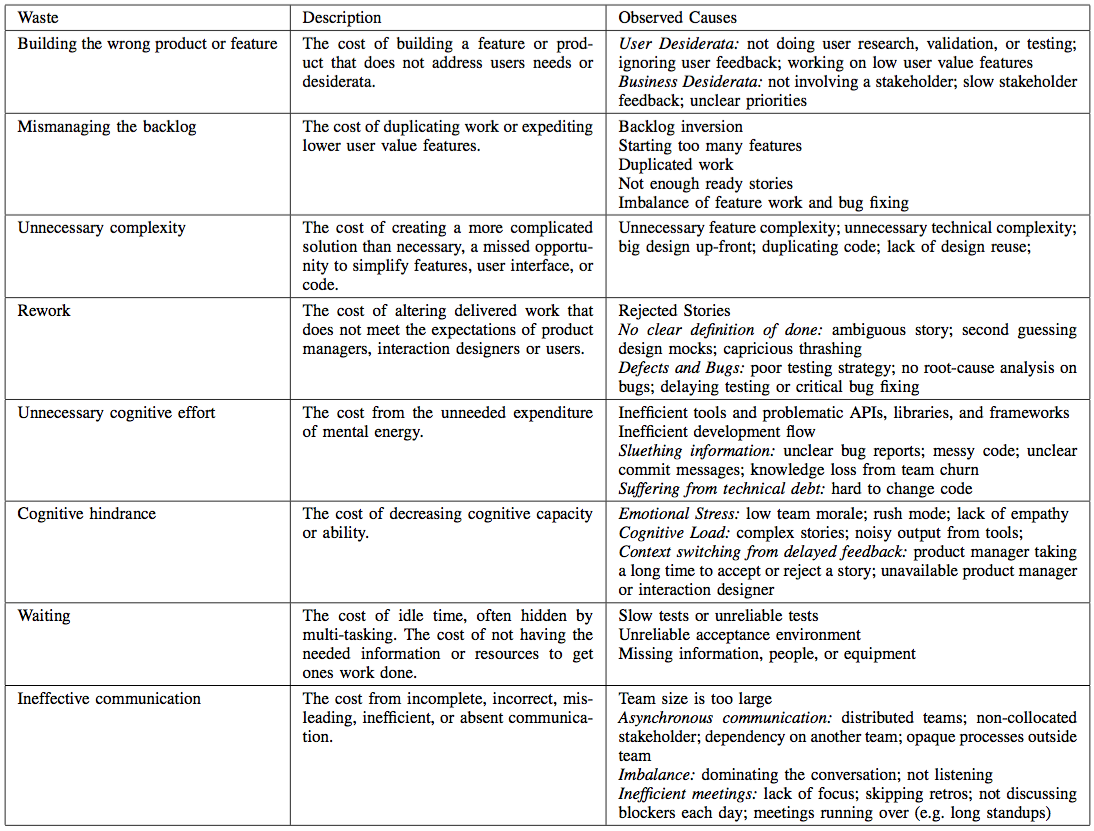
\includegraphics[width=6.4in]{software_engineering_waste/waste.png}
\end{figure}

% \begin{table*}[t]
% \renewcommand{\arraystretch}{1.3}
% \centering
% \caption{Types of Software Development Waste}
% \label{Waste}
% \begin{tabular}{|p{1.5in}|p{1.6in}|p{2.8in}|} %dissertation size
% \hline
% Waste                                 & Description                                                                                                         & Observed Causes                                                                                                                                                                                                                                                                                                                                                                                                                     \\ \hline
% Building the wrong product or feature & The cost of building a feature or product that does not address user’s needs or desiderata.                                  & \textit{User Desiderata:} not doing user research, validation, or testing; ignoring user feedback; working on low user value features \newline \textit{Business Desiderata:} not involving a stakeholder; slow stakeholder feedback; unclear priorities                                                                                                                                                                                  \\ \hline
% Mismanaging the backlog               & The cost of duplicating work or expediting lower user value features.                                                       & Backlog inversion \newline Starting too many features \newline Duplicated work \newline Not enough ready stories  \newline Imbalance of feature work and bug fixing                                                                                                                                                                                                                                                                                                                                      \\ \hline
% Unnecessary complexity  & The cost of creating a more complicated solution than necessary,  a missed opportunity to simplify features, user interface, or code.      & Unnecessary feature complexity; unnecessary technical complexity; big design up-front; duplicating code; lack of design reuse;                                                                                                                                                                                                                                                                                                                 \\ \hline
% Rework                                & The cost of altering delivered work that does not meet the expectations of product managers, interaction designers or users.    & Rejected Stories \newline \textit{No clear definition of done:} ambiguous story; second guessing design mocks; capricious thrashing \newline \textit{Defects and Bugs:} poor testing strategy; no root-cause analysis on bugs; delaying testing or critical bug fixing                                                                                                                                                                    \\ \hline
% Unnecessary cognitive effort          &   The cost from the unneeded expenditure of mental energy.                                                                                                                 & Inefficient tools and problematic APIs, libraries, and frameworks  \newline Inefficient development flow \newline \textit{Sluething information:} unclear bug reports; messy code; unclear commit messages; knowledge loss from team churn \newline\textit{Suffering from technical debt:} hard to change code
%                                                                      \\ \hline
% Cognitive hindrance           & The cost of decreasing cognitive capacity or ability.                        & \textit{Emotional Stress:} low team morale; rush mode; lack of empathy \newline \textit{Cognitive Load:} complex stories; noisy output from tools; \newline \textit{Context switching from delayed feedback:} product manager taking a long time to accept or reject a story; unavailable product manager or interaction designer                                                                                                                                                        \\ \hline
% Waiting                               & The cost of idle time, often hidden by multi-tasking. The cost of not having the needed information or resources to get one’s work done. & Slow tests or unreliable tests \newline Unreliable acceptance environment \newline Missing information, people, or equipment                                                                                                                                                                                                                                                                            \\ \hline
% Ineffective communication             & The cost from incomplete, incorrect, misleading, inefficient, or absent communication.                         & Team size is too large \newline \textit{Asynchronous communication:} distributed teams; non-collocated stakeholder; dependency on another team; opaque processes outside team \newline \textit{Imbalance:} dominating the conversation; not listening \newline \textit{Inefficient meetings:} lack of focus; skipping retros; not discussing blockers each day; meetings running over (e.g. long standups) \\ \hline                  
% \end{tabular} 
% \end{table*}

We identified eight types of waste listed in Table \ref{Waste}. The table lists the waste type, a description, and observed causes. For the Cognitive Hindrance Waste, Figure \ref{ChainOfEvidence} shows the waste category, its cause categories and properties and examples. Appendix \ref{AppendixChainOfEvidence} presents the entire chain of evidence.

This section defines, elaborates, and provides examples of each waste type. When observed, we provide tensions with respect to the waste.

\subsection{Waste: Building the wrong feature or product}
Building features (or worse, whole products) that no one needs, wants, or uses obviously wastes the time and efforts of everyone involved. We observed this waste affecting team morale and team code ownership \cite{SedanoTeamCodeOwnership}. Clearly, this can affect customer satisfaction. 

The product features for Project Ses were designed based on a given persona\textemdash i.e. a fictional, archetypal user \cite{Grudin2002personas}. However, consulting several real intended users revealed that the persona was deeply flawed as the users did not need the product, (the intended users invalidated the persona.) Building the intended product would have been risky and probably wasteful. 

\textbf{Tension: User needs} versus \textbf{business wants.}
Some projects exhibit a tension between user needs and business goals. Practitioners may struggle to produce something that simultaneously satisfies the users and the business.

For example, on Project Quattuor, the client wanted to add a news feed to a mobile phone application that controlled a real world product. However, user validation revealed that no users wanted this feature, and several reacted quite negatively. Despite numerous conversations, the marketing department insisted on adding the feature. 
\subsection{Waste: Mismanaging the backlog}
A product backlog can be mismanaged in several ways, leading to delays of key features or lower team productivity. 

For example, we observed engineers on several projects working on low-priority stories through \quotes{backlog inversion.} This occurs when the engineers working through the backlog get ahead of the project manager who is prioritizing the backlog. For instance, the product manager might prioritize the next ten stories in the backlog, but the engineers get to story 15 before the product manager gets back to prioritizing. This creates waste as engineers implement potentially outdated, low-value, or even counterproductive stories ahead of high-value stories.   

Mismanaging the backlog can also lead to duplicated work in at least three ways. For example, we observed duplicated stories in the backlog, two engineers working on the same story because one had forgotten to change its status in the backlog software (Pivotal Tracker), and two engineers independently addressing the same pain point (e.g. making the build faster) by not adding chores to reflect their work in progress.

\textbf{Tension: Writing enough stories} versus \textbf{writing stories that will never be implemented.}
Pivotal product managers attempt to provide the team with a steady stream of ready, high-value work. This creates a tension between writing enough stories for the team to work on and \quotes{over-producing} stories that might never be implemented. Writing too few stories wastes the team's time while writing too many stories wastes the product manager's time. We observed teams running out of work on rare occasions; we did not observe product managers writing too many stories.  

\textbf{Tension: Finishing features} versus \textbf{starting too many features.}
Product managers decompose a feature into a set of stories, and typically sequence the stories to finish just enough of each feature before starting another feature in order to create the minimal viable product as soon as possible. 

On Project Quattuor's backend system, we observed one product manager starting too many tracks of work at once by prioritizing a breadth of features instead of finishing started features. Unfortunately, several tracks of work were not completed by the first release date. The work in progress was disabled with feature flags. Starting work, changing priorities, and halting work in flight, can result in waste.

Pivotal prefers to maintain a shippable product while finishing minimal viable product versions of each feature as soon as possible. 

\subsection{Waste: Unnecessary complexity}
\textit{Unnecessary complexity} can be caused by complex features (which reduces the user's satisfaction), technical complexity, and unnecessary unique interaction designs (both of which reduces the team's productivity.) 

When a product or feature is unnecessarily complex, it wastes users' time, especially when users struggle to understand how to apply it to achieve their objectives. The anfractuous product is difficult to use. Some features bring unnecessary technical complexity as a simpler interaction design would have solved the same problem. %\sout{We observed a simple solution was to increase conversations with product, design, and engineering. On one project, an engineer shortened the feedback loop by daily checking-in with the interaction designer.}

Similarly, an unnecessarily technical complexity wastes developers' time with unduly difficult to build and maintain code. On Projects Tes, Ses, and Septem, complicated legacy components were refactored into simpler, easier to understand components. Sometimes personal goals do not align with the team goals leading to unnecessary complexity. A Pivotal engineer said that a client engineer's attitude was, \participantQuote{the more complicated, the better, as that means my role is the more important.}

Another way to increase system complexity is through unnecessary uniqueness, i.e., building a new component instead of reusing an existing component. In code, unnecessary uniqueness manifests as duplicated code. In mockups, unnecessary uniqueness results in \quotes{design snowflakes} which could take advantage of design reuse. On Project Duo, the interaction designer created a left-to-right navigational flow for configuring the product but designed a top-to-bottom navigational flow for the checkout page. Both sequences allowed the user to change a previous choice, jump to the correct page, and invalidate dependent information. In retrospect, development time would have shortened if both used the same design treatment. On Project Quattuor, the presence of multiple designers resulted in different design treatments for the same concept. The product shipped multiple versions of layouts, lists, alerts, and buttons, some with expensive interactions to engender user delight. On Project Kvin, the interaction designer created two sets of form inputs which necessitated multiple CSS styles for the HTML form input tags. Singular designs require engineering to build unique solutions with no possibility of reuse.   

\textbf{Tension:  Big design up-front} versus \textbf{incremental design.}
Many projects exhibit a tension between up-front and incremental design. Rushing into implementation can produce ineffective emergent designs, leading to expensive rework. However, big up-front design can produce incorrect or out-of-date assumptions and inability to cope with rapidly changing circumstances, also leading to expensive rework. The desire to avoid rework and differing development ideologies, therefore, motivate tension and disagreement over big design up-front versus incremental design. 

The observed teams expected the product features to change even when the client had clearly defined the project. On all projects with interaction designers, after the interaction designer conducted user research and discovered new information about the user's needs, the feature set changed. No amount of up-front consideration appears sufficient to predict user feedback. The Pivotal teams preferred delivering functionality incrementally and delay integrating with technologies until a feature requires it. For example, an engineer would only add asynchronous background jobs technology when working on the first story to require the needed technology, even if the team knew it would need it on day one of the project.

We observed teams using common architectural and design solutions from similar, previous projects without explicit architectural or design phases.
\subsection{Waste: Rework}
In this study, participants distinguish between rework, revising delivered work that was not done correctly, and new work, improving existing work based on new information. For example, improving a feature based on new user feedback is new work, while rewriting a buggy test case is \textit{rework}.  \textit{Rework}, by definition, wastes resources and developer time. 

We observed numerous sources of \textit{rework} including stories with no clear definition of done, rejected stories, defects in the code, poor testing strategy, ambiguous mock-ups, and delaying testing or critical bug fixing.

On Project Ses, the engineers showed a finished story to the interaction designer for feedback. The interaction designer pointed out a missing interaction, yet the desired behavior was not in the story and not described in the mock-up.

On Project Quattuor, the client delayed fixing of critical bugs until just before the release. Fixing one bug in the backend system had a cascading effect with the clients which expected the code to work a certain way. \textit{Rework} could have been avoided had the critical bug been fixed prior to the client code becoming dependent on it.

On Project Quattuor, the interaction designers created mockups optimized for English, not the target language. After implementing the application, the team realized that the primary foreign language translation took up more space than the English translations, requiring rework for several design components. 

On Project Kvin, the interaction designer did not consider a responsive web design for mobile phones when building the mock-ups. After building a few screens, the team realized that the website did not work well on mobile devices requiring \textit{rework}.

\textbf{Tension: Responding to change} versus \textbf{thrashing.}
While the ability to respond to change quickly is a core tenet of agile development; time, effort, and resources can still be wasted by changing features too often (thrashing). Here, we are trying to distinguish between rapidly improving a product based on new information and repeated, capricious tweaking. 

On Project Kvin, for example, the launch was delayed while the business fiddled with the sequence and number of steps in the user registration process. Project Duo was similarly delayed by a project manager repeatedly resequencing an order customization process. 


% \sout{A related tension is initial velocity versus avoiding rework, that is, the where developers commit code knowing it will need rework to make this sprint's deadline. Reworking the code becomes a story for a future sprint. This is a good example of counterproductive incentives and how workplace monitoring leads to performances that reduce productivity. Is this the kind of thing we want to talk about here? If not, maybe we can cut this tension.}

\subsection{Waste: Unnecessary cognitive effort}
When team members or users have \textit{unnecessary cognitive effort}, their energy and time are wasted. \textit{Unnecessary cognitive effort} includes the waste from sleuthing missing information, knowledge loss from team churn, suffering from technical debt, inefficient tools, and problematic APIs.

We observed several instances of engineers sleuthing for needed information when, for example, code and commit messages did not convey intention, or bug reports were incomplete. Similarly, in projects where knowledge silos formed, team churn leads to wasted effort regaining lost knowledge. Context switching creates similar time and effort waste (see \textit{waiting} waste description for more detail). 
 
Technical debt refers to delaying needed technical work, by taking technical shortcuts, usually to meet a deadline \cite{McConnellTechnicalDebt}. We observed teams suffering from technical debt with long-running, existing code bases. On Project Tes, running the test suite produced 87,000 lines of output including deprecation warnings, exceptions, and test noise. Engineers ignored the overwhelming output which contained important information. With considerable effort, the team fixed the test output to only contained test failures. On Project Ses, dead code littered the code base along with convoluted objects. Project Septem suffered from engineers introducing an idea in one part of the code base, but not applying the concept systematically. The project had multiple CSS themes, multiple test suites using different programming languages, multiple naming conventions, and multiple ways of interacting with the data repositories. On each of these projects, the teams spent considerable effort paying down technical debt to improve their productivity and team code ownership \cite{SedanoTeamCodeOwnership}.  

On Project Quattuor, the product managers were busy managing up as well as providing enough stories to keep the teams occupied. As a result, product managers frequently delayed accepting and rejecting stories. Developers might restart a rejected stories they finished awhile ago requiring them to recall the context around the story. The team followed pair rotation from sustainable software development \cite{SedanoSustainableSoftware} which meant that the pair picking up a rejected story was probably not the pair that worked on it.

In several projects, meanwhile, we observed ineffective tooling (development environments, deployment processes) and convoluted, nonfunctional, premature, complicated, unstable, outdated, unsupported, time-consuming, or inappropriate-for-the-task software libraries leading to engineers working ineffectively. One frustrated software engineer said that one arcane technology \participantQuote{makes me angry enough that I want to hack into it, expose how useless and horrible it is and wipe this miserable product off the face of the earth!}
\subsection{Waste: Cognitive hindrance}
\textit{Cognitive hindrance} is anything that decreases the cognitive capacity and cognitive ability, much like a \quotes{debuff} from role playing games. This waste decreases the person's individual productivity. We particularly observed productivity problems related to emotional stress, cognitive load, and context switching.

On Project Quattuor, for example, the team rushed to release a fixed feature set by a fixed date. They even had a countdown to the release date on an office whiteboard. We observed low team morale, rush mode, lack of empathy, and waiting too long to resolve interpersonal issues leading to people working inefficiently. The team furthermore felt that over-emphasizing the deadline was increasing stress and leading to poor technical decisions, and eventually erased the countdown from the whiteboard. Participants felt that fixing both scope and schedule was antithetical to Pivotal's software process, where the client either chooses the release date and gets the features ready by then or chooses key features and ships the product when the features are ready. 
\subsection{Waste: Waiting}
Having developers waiting around, working slowly or working on low-priority features because something is preventing them from proceeding on high-priority features wastes their time. For example, we observed developers waiting on (or looking for) product managers and designers to clarify a story's acceptance criteria. On Project Quattuor, product managers started multitasking while accepting stories because the acceptance environment was unreliable. We saw team members waiting around because of missing video-conferencing equipment. 
Ohno described \textit{waiting} waste as hidden waste since people start working on the next job, instead of waiting \cite{OhnoToyotaProductionSystem}. To expose this waste, in Toyota Production System, when someone pulls the red cable, everyone stops, bringing attention to the waste. On Project Ses, engineers were waiting hours for the build. It took 58 minutes to run locally and 17 minutes on the build machine due to parallelization on four machines. Team members would not run tests locally, but push code as a branch to the build machine. While the build machine ran the tests, the engineers would either wait or context switch onto different work. If the branch passed, some time later, they would merge their code into the team's code. If the branch failed, the engineers would decide to finish the work that they were doing or switch back and fix the issue. Some engineers found the context switching exhausting. The \quotes{sollution} for \textit{waiting} created \textit{cognitive hindrance} waste.

\textbf{Tension: Wait, block or guess.}
When needed information is missing, engineers appear to have three options: 1) wait for the information; 2) suspend (block) the story and work on something else; 3) act without the information. The best option depends on how far into the story the pair is, how long they have to wait, and their confidence in their best guess.

\textbf{Tension: Waiting} versus \textbf{context switching.}
While engineers are waiting, they often work on something else. However, task switching decreases productivity and increases mistakes \cite{MonsellTaskSwitching}. For short waits, it is therefore probably less wasteful for engineers to just take a break like play table tennis than to switch to another work task. 

\subsection{Waste: Ineffective communication}
\textit{Ineffective communication} is the cost from incomplete, incorrect, misleading, inefficient, or absent communication. We observed large team sizes, asynchronous communication, imbalance in communication, and inefficient meeting reducing team productivity.

We observed issues with asynchronous communication on Project Quattuor. The team was distributed between two offices located an hour apart. We observed the team using remote pairing and engineers commuting between the offices to mitigate the effects of a large distributed team. Even still, communication issues were a perennial theme in the retrospections.


On Project Ses, we observed that one person dominated meetings which prevented quieter personalities from sharing their perspective. 

On Project Quattuor, when the project started, the iOS team did not have a retro and was also lacking a way to make decisions. Adding weekly retros enabled the team to reflect and respond to problems. Over several weeks, the remaining teams added their own retro. 

%When teams are not co-located, additional time is spent on asynchronous communication. Instead of dialoguing about an issue, time is spent crafting a message, sending it, waiting for a response, and interpreting the response. When the message is misunderstood, resolving it takes longer than synchronous communication. When the team is distributed, it loses the benefits of osmotic communication.

%Increasing team size increases the number of communication paths. The number of paths is N x (N -1) / 2. 


% On Project Quattuor, \participantQuote{not enough listening in iOS technical meeting} appeared in two retros. 

% \textit{Ineffective communication} is a well studied topic. \cite{LencioniDeathByMeeting, CollaborationExplained, TabakaCollaborationExplained}.

\section{Comparing to Lean Software Development}
\label{LeanSoftwareDevelopmentComarison}

This section compares our taxonomy of software engineering waste presented in Section \ref{SEWaste}, with Lean Software Development's taxonomy of waste. The goal is to not to critique either model, but to see how the software engineering waste model incorporates features of the Lean Software Development model \cite{PoppendieckConceptToCash}. 

\quotes{It is incumbent upon the researcher to compare and show the variations as different properties under different conditions and then integrate them. \ldots The job is to generate, not verify} \cite{GlaserTheoreticalSensitivity}. 


\begin{table}[t]
\renewcommand{\arraystretch}{1.5}
\centering
\caption{Comparison to Lean Software Development Waste}
\label{LeanSoftwareDevelopmentComparison}
% \begin{tabular}{|p{1.57in}|p{1.57in}|}
\begin{tabular}{|l|l|}
\hline
Software Development Wastes           & Poppendiecks' Software Development Wastes \\ \hline
Building the wrong product or feature & Extra features                            \\ \hline
Mismanaging the backlog               & Partially Done Work                            \\ \hline
Unnecessary complexity                & Not described                             \\ \hline
Rework                                & Defects                                   \\ \hline
Unnecessary cognitive effort          & Relearning                             \\ \hline
Cognitive hindrance           & Task switching                             \\ \hline
Waiting                               & Delays                                    \\ \hline
Ineffective communication             & Not described                             \\ \hline
Not observed                          & Handoffs                                  \\ \hline
\end{tabular}
\end{table}
\subsection{Common to both models}
\textbf{Building the wrong feature} and \textbf{Extra features}: In our model, \textit{building the wrong feature} describes building low-value features for the user. Pivotal's process relies on user validation to assess value in solving the user's needs and iterating from a minimal viable product. In Lean Software Development, \textit{extra features} describes adding in features that are not yet necessary for the product. Lean Software Development mentions the cost of managing, implementing, compiling, integrating, testing, and maintaining unneeded code \cite{PoppendieckLeanSoftwareDevelopment}.  Both perspectives align on delaying features until necessary. 

\textbf{Mismanaging the backlog} and \textbf{partially done work}: In our model, \textit{mismanaging the backlog} represents sequencing low priority work before high priority work or accidentally duplicating work. In Lean Software Development, \textit{partially done work} is work that is not tested, implemented, integrated, documented, or deployed. Any feature description that is not implemented, any code that is not integrated or merged, any code that is untested, any code that is not self-documenting or documented, and any code that is not deployed where the user can receive value is \textit{partially done work}.

In observing Pivotal, teams do not view materials flowing through the system as waste. Interaction designers need to be producing just enough mockups, product managers need to be writing just enough stories, the developers need to be writing just enough code to make the story work. In any continuous flow system, there is unfinished materials at each step. 

While we did observe a product manager that started too many features at once (as described in \textit{mismanaging the backlog} waste section), we mostly observed work flowing in a relatively orderly fashion as compared to a waterfall software process. If we were to observe large amount of waiting designs, or large amounts of waiting stories, then we would classify that waste as \textit{mismanaging the backlog}.

There is common ground between both models on reducing large batch sizes into smaller batches with an ideal of  \quotes{continuous flow,} where work is routinely moving through the system. 

\textit{Mismanaging the backlog} describes observed wastes not covered by \textit{partially done work.}

%Just-in-time production is antithetical to large batch sizes. In any continuous flow system, there is unfinished materials at each step. 

%Based on this understanding of continuous flow, we believe that \textit{\partially done work} is suggesting that large batch sizes need reducing.   

%The Toyota Production System creates buffers of parts at certain steps in the pipeline, like a bumper sits waiting to be used on the next car. Once that bumper is consumed, the process of creating another bumper just like it is started. Enough material is produced to keep continuous flow moving. Ohno was concerned about the stockpiles of inventory stored in warehouses.

%Since Pivotal engineers follow Test Driven Development / Behavior Driven Development, strive to get the tested code into the developer's master branch as quickly as possible, and release frequently, we did not observe the waste associated with partially done work. At any moment in time, an interaction designer is creating a future mock, a product manager is updating a future story, a developer is testing code that has not shipped. This describes the continuous flow of features to the customer. 

\textbf{Rework} and \textbf{Defects}: In our model, \textit{rework} includes mistakes made by the product managers (in writing acceptance criteria), the interaction designers (in creating mockups) and the developers (in writing tests and code). Poor testing strategies, and delaying testing can cause rework. In Lean Software Development, \textit{defects} are the coding mistakes of developers. Therefore the two models align on \textbf{defects} and our model broadens the waste definition with \textit{rework}. \textit{Rework} is a superset of \textit{defects}. 

\textbf{Unnecessary cognitive effort} and \textbf{Relearning}: In our model, \textit{unnecessary cognitive effort} includes the waste from sleuthing for missing information, knowledge loss from team churn, and suffering from technical debt. In Lean Software Development, \textit{relearning} is \quotes{rediscovering something we once knew} \cite{PoppendieckConceptToCash}. Included in \textit{relearning} is failing to engage people in the development process. We did observe product managers having difficulty in involving certain stakeholders, which we include in the \textit{building the wrong product or feature} waste. \textit{Relearning} is only one form of \textit{unnecessary cognitive effort}.

\textbf{Cognitive hinderance} and \textbf{Task switching}: In our model, \textit{cognitive hinderance} includes the waste from emotional stress, cognitive load, and context switching. In Lean Software Development, \textit{task switching} is the cost from trying to multitask or work on more than one task at a time. (Based on our analysis, task switching appears to be a cause, not a waste type.) The desire to have developers work on one thing at a time is common to both models. \textit{Cognitive hinderance} is a superset of \textit{task switching}.  

\textbf{Waiting} and \textbf{Delays}: In our model, \textit{waiting} includes delays from not having the needed information or resources to get one's work done as well as the cost of slow tests and unreliable tests. In Lean Software Development, \textit{delays} are \quotes{waiting for people to be available who are working in other areas} to provide needed information that is not available to the developers. \cite{PoppendieckConceptToCash}. Both wastes describe the cost of missing needing information. \textit{Waiting} is a superset of \textit{delays}.
\subsection{Observed only in Lean Software Development}

\textbf{Handoffs}: \textit{Handoff} waste is the loss of tacit knowledge when work is handed off to colleagues.

We did not observe this as Pivotal follows an iterative software development process with cross functional teams. We did observe \textit{waiting} waste as engineers might contact people outside the team who had needed information. If we were to observe handoffs, then we would classify the subsequent waste as \quotes{sleuthing information} as part of \textit{unnecessary cognitive effort.} 
\subsection{Observed only in our model}
The analysis revealed that Lean Software Development waste taxonomy does not handle the following waste types: \textit{Unnecessary complexity}, and \textit{Ineffective communication}. This suggests that the taxonomy needs expanding to cover our observed cases of waste. For more detail about each of the wastes, see Section \ref{SEWaste}.
\section{Results Evaluation}
\label{ResultsEvaluation}
While other factors may affect software engineering waste, we focus only on those that we observed during the study. Grounded Theory studies can be evaluated using the following criteria \cite{Charmaz, StolGroundedTheory}:
\textbf{Credibility}: \quotes{Is there sufficient data to merit claims?}  This study relies on two years of participant-observation, \numberOfInterviews{} intensive open-ended interviews, and the agenda of one year's worth of retrospections. 
\textbf{Originality}: \quotes{Do the categories offer new insights?}  This is the first study of waste in software development based on empirical evidence. Prior work is anchored in concepts from manufacturing which might force the model with preconceived ideas. 
\textbf{Resonance}: \quotes{Does the theory make sense to participants?} Several participants reviewed our findings and indicated that the waste taxonomy resonates with their experience.
\textbf{Usefulness}: \textbf{Does the theory offer useful interpretations?} This study acknowledges software development wastes that are not identified in manufacturing. This study explains why certain behaviors, events, and actions can cause software engineering waste. This study provides a rich waste taxonomy for Value Stream Mapping in software development. 

This work analyzed software projects at the Silicon Valley office of Pivotal following Extreme Programming. From an \textbf{external validity} perspective, grounded theory is non-statistical, non-sampling research. The results, therefore, cannot be statistically generalized to a population. Rather, researchers and professionals can adapt the concepts and ideas to other contexts case-by-case.

Finally, the results might be influenced by \textbf{researcher bias} or \textbf{prior knowledge bias}. A risk of the participant-observer technique is that the researcher may lose perspective and become biased by being a member of the team. While a participant-observer gains perspective an outsider cannot, an outside observer might see something a participant observer will miss. Similarly, while prior knowledge helps the researcher interpret events and select lines of inquiry, prior knowledge may also blind the researcher to alternative explanations \cite{GlaserIssues}. We mitigated these risks by recording interviews and having the second and third authors review the coding process and reviewed the detailed retro topics.

Since Pivotal follows iterative software development, we did not observe wastes commonly associated with the waterfall approach. We know that \textit{waiting} waste is present in other organizations that hand feature documents from one team to another team or use large batch sizes of features \cite{Ali2016, Khurum2014, Mujtaba2010}.

Pivotal has relied on Extreme Programming for almost two decades. While Pivotal attempts to remove waste whenever possible, as a \quotes{lean} software development organization, there may be additional wastes not observed in this research study. 
\section{Conclusion}
\label{Conclusion}
We present the first evidence-based taxonomy of software engineering waste, identifying several waste types together with their causes and tensions. Each waste is illustrated with examples taken from observed projects at Pivotal, showing how the waste materializes, and in some cases how it is removed or eliminated. We also compare our proposed taxonomy to the one found in Lean Software Development.

The proposed taxonomy emerged from a Constructivist Grounded Theory research, including the collection and analysis of data coming from \durationOfResearchStudyPlural{} of participant-observation of \numberOfObservedProjects{} software development projects, interviews of \numberOfInterviews{} software engineers, interaction designers, and product managers, as well as one year of retrospection topics. The analysis of the retrospection topics reveals that the observed Pivotal teams care very much about finding and eliminating wastes in their software development process. The retrospection topics are a treasure trove illustrating many different types of waste. 

Contrary to the Lean Software Development's taxonomy of wastes, which is top-down because created by mapping manufacturing wastes to software wastes, our taxonomy is bottom-up as it is grounded in empirical data. The comparison of the two models shows some alignment. However, our taxonomy expands the Lean Software Development's taxonomy by broadening the definition of most wastes and introducing additional wastes not previously identified. As such, our taxonomy is more expressive and more accurately describes the observed data.

Future research includes continuing to validate the resonance of the proposed waste taxonomy with additional participants at Pivotal. This might involve collecting more data and evolving the taxonomy accordingly. Also, we would like to investigate how Pivotal relies on feedback loops as a mechanism for identifying, dealing with, and reducing waste. 

%\sout{At the core of Lean Thinking is waste identification and elimination \cite{WomackLeanThinking} which is a key differentiator between Lean and Agile in software development \cite{Fitzgerald2015continuous}. (Agile does promote the use of feedback loops which we observed as a common solution for waste identification and removal at Pivotal.)

%Ohno and Shingo singularly focused on the efficiency of the production line through continuous waste removal. By excluding product development activities, the design of the vehicle, they overlooked the entire picture. This may explain why their waste taxonomy misses aspects fundamental to product design.

%In applying waste removal to software development, it behooves the software community first to start with a waste taxonomy grounded in data from software development, not borrow from a dissimilar domain. Since waste removal is core to the Lean movement, starting with an ill formulated waste taxonomy suggests a possible fundamental impact on Lean Software Development claims.

%This work suggests that evidence-based research yields insights grounded in data that have not emerged from applying manufacturing concepts to software development.}

%\sout{Based on the research from value stream mapping, the first step of waste reduction may be switching a software firm from a batch-and-pull process where a feature document is handed to a team to implement (e.g. a waterfall system) to a system where a small number of features are handed to a team (e.g. iterative software development.) Then introducing and reducing feedback loops to remove additional waste.}
% \section*{Acknowledgement}
% Thanks to Ben Christel for his assistance in sorting retro topics and helping with the initial analysis. Thank you to Rob Mee, David Goudreau, Ryan Richard, and Zach Larson for making this research possible.


